
\section{The model}
\subsection{Building network}

\begin{frame}[b]{Our proposed model}
	\centering
	Following, we will present the proposed model of this work\\[10em]
	
	\setbeamercovered{invisible}
	\onslide<+(1)->{%
	\begin{itemize}
		\item How to build a \textbf{network} from roll-call \textbf{votes}?
		\item Elaboration of \textbf{two spin systems} and their respective statistical mechanical properties.
\end{itemize}}
\end{frame}

\subsection{Building a network from roll-call votes}
\begin{frame}[b]{Building a network}{From votes to connections}
	\foreach \n in {1,...,5}{
		\only<\n>{%
		\begin{tikzpicture}[remember picture, overlay]
			\node[at=(current page.north), anchor=north, shift=({-5mm,-5mm})] {
				\includegraphics[width=1.1\columnwidth]{netbuild-step-\n.pdf}
			};
		\end{tikzpicture}
		}
	}
	\begin{tikzpicture}[remember picture, overlay]
		\node[at=(current page.north east), anchor=west,shift=({-25mm,-21mm})] {\small For};
		\node[at=(current page.north east), anchor=west,shift=({-25mm,-27mm})] {\small Against};
		\node[at=(current page.north east), anchor=west,shift=({-25mm,-32mm})] {\small Abstained};
	\end{tikzpicture}
	\onslide<2->
	\begin{itemize}[<+(2)->]
		\item For a given vote, we connect all legislators with each others.
		\item Legislators that voted the {\color{blue}same} are connected with a {\color{blue}positive} link.
		\item<.(2)-> Legislators that voted {\color{red}different} are connected with a {\color{red}negative} link.
	\end{itemize}
\end{frame}

\begin{frame}[b]{How to identify a vote configuration?}
		\only<+->{%
		\begin{tikzpicture}[remember picture, overlay]
			\node[at=(current page.north), anchor=north, shift=({-5mm,-5mm})] {
			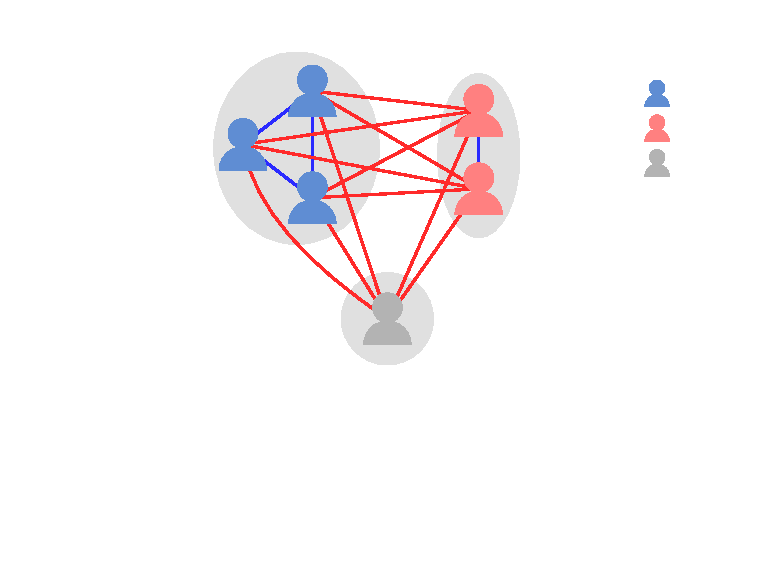
\includegraphics[width=1.1\columnwidth]{netbuild-step-5.pdf}
			};
		\end{tikzpicture}
		}
	\begin{tikzpicture}[remember picture, overlay]
		\node[at=(current page.north east), anchor=west,shift=({-25mm,-21mm})] {\small For};
		\node[at=(current page.north east), anchor=west,shift=({-25mm,-27mm})] {\small Against};
		\node[at=(current page.north east), anchor=west,shift=({-25mm,-32mm})] {\small Abstained};
	\end{tikzpicture}
	\onslide<+->{%
	\begin{tikzpicture}[remember picture, overlay]
		\node[at=(current page.north east), anchor=west,shift=({-11mm,-21mm})] {\small $=3$};
		\node[at=(current page.north east), anchor=west,shift=({-11mm,-27mm})] {\small $=2$};
		\node[at=(current page.north east), anchor=west,shift=({-11mm,-32mm})] (uno) {\small $=1$};
		\node[draw,red,at=(current page.center), anchor=west,shift=({13mm,-7mm}),outer sep=1mm] (vec) {\color{black}$\vec{n}=\{3,2,1\}$};
		\draw[-stealth,red] (uno.south) to[out=-110,in=0] (vec.east);
	\end{tikzpicture}}
	\begin{itemize}
		\item Our system of interest is \textbf{completely} defined by the amount of legislators that backed each vote option. 
	\item Any vote can be represented as a vector
\begin{equation}
	\vec n = \{n_1, \ldots,n_{k}\}.
\end{equation} 
\end{itemize}
\end{frame}

\begin{frame}{Vote configurations}
	Note that, for $k$ vote options and a fixed $N$ number of legislators, 
	\begin{equation}
		\sum_i^k n_i = N\label{eq:Ni_sum}
	.\end{equation}
	This equation define a space where all possible configurations the system could be in live. 
\end{frame}

\begin{frame}{Configuration space}
	\setlength{\fboxsep}{0pt}
	\setlength{\fboxrule}{0pt}
	\begin{center}
		\fbox{%
		\adjincludegraphics[trim={{0.0\width} {0.03\height} {0.0\width} {0.02\height}},
							clip,
							height=0.83\textheight]
						{figs-poster/phasespace_plane}}
		\label{fig:cf}
		\captionof{figure}{Configuration space for $k=3$ and $N=155$. The axes $n_1,n_2$ and $n_3$ represent the amount of support for such vote option.}
	\end{center}
\end{frame}

